\documentclass{article}
\usepackage[a4paper, total={7in, 9in}]{geometry}
\usepackage[brazil,portuges]{babel}
\usepackage[utf8]{inputenc}
\usepackage[T1]{fontenc}
\usepackage{ebgaramond}
\usepackage{amsmath}
\usepackage{indentfirst}
\usepackage{titlesec}
\usepackage{todonotes}
\usepackage{enumitem}
\usepackage{tikz}
\usepackage{array}
\usepackage{multirow}
\usepackage{listings}% http://ctan.org/pkg/listings
\lstset{
  basicstyle=\ttfamily,
  mathescape
}
% oi abiguinhos %
\title{Compiladores - Prova 2}
\author{André L. Mendes Fakhoury\\
Gustavo V. V. Silva Soares\\
Eduardo Dias Pennone\\
Matheus S. Populim\\
Thiago Preischadt\\
}
\date{2021}

\begin{document}

\maketitle

\section{Considere a gramática simples abaixo:}
\begin{lstlisting}
<A> ::= ( <B> ) | x
<B> ::= <A> , <B> | <A>
\end{lstlisting}

\subsection{(a) Considerando a análise ascendente de precedência de operadores, mostre passo a passo a construção da tabela sintática pelo método mecânico.(Calcule primeiros e últimos, relações <, > e = de operadores e construa a tabela sintática).}

A linguagem é de precedência de operadores e não ambígua.

Os primeiros terminais de <A> são $\{(, x\}$ e os últimos são $\{), x\}$.

Os primeiros e os últimos terminais de <B> serão os mesmos de <A>.

A partir dos pares do tipo $aX$, que são $( <B>$ e $, <B>$, podemos extrair as seguintes relações: $( < ($, $( < x$, $, < ($ e $, < x$.

A partir dos pares do tipo $Xb$, que são $<B> )$ e $<A> ,$, podemos extrair as seguintes relações: $) > )$, $x > )$, $) > ,$ e $x > ,$.

A partir da sequência do tipo $a\beta b$, que é $( <B> )$, podemos extrair a seguintes relação: $( = )$.

Também temos que $\$ < ($, $\$ < x$, $) > \$$ e $x > \$$.

A tabela sintática é:
\begin{center}
\begin{tabular}{ |c|c|c|c|c|c| } 
\hline
  & ( & ) & x & , & \$ \\
\hline
( & < & = & < &   &  \\
\hline
) &   & > &   & > & >\\
\hline
x &   & > &   & > & >\\
\hline
, & < &   & < &   &  \\
\hline
\$ & < &   & < &   &  \\
\hline
\end{tabular}
\end{center}

\subsection{(b) Considerando a análise ascendente SLR, construa passo a passo a tabela sintática.}
Utilizaremos a gramática equivalente:
\begin{lstlisting}
(01)  <S> ::= <A>
(02)  <A> ::= ( <B> )
(03)  <A> ::= x
(04)  <B> ::= <B> , <A>
(05)  <B> ::= <A>
\end{lstlisting}

O conjunto canônico de itens LR(0) da linguagem é:
\begin{lstlisting}
(01)  <A> ::= .( <B> )
(02)  <A> ::= (. <B> )
(03)  <A> ::= ( <B>. )
(04)  <A> ::= ( <B> ).
(05)  <A> ::= .x
(06)  <A> ::= x.
(07)  <B> ::= .<B> , <A>
(08)  <B> ::= <B>. , <A>
(09)  <B> ::= <B> ,. <A>
(10)  <B> ::= <B> , <A>.
(11)  <B> ::= .<A>
(12)  <B> ::= <A>.
(13)  <S> ::= .<A>
(14)  <S> ::= <A>.
\end{lstlisting}

Com isso podemos construir o seguinte AFND.
\begin{center}
\begin{tikzpicture}[scale=0.2]
\tikzstyle{every node}+=[inner sep=0pt]
\draw [black] (17.8,-18.6) circle (3);
\draw (17.8,-18.6) node {$A$};
\draw [black] (29.5,-18.6) circle (3);
\draw (29.5,-18.6) node {$1$};
\draw [black] (17.8,-8.1) circle (3);
\draw (17.8,-8.1) node {$5$};
\draw [black] (58.5,-18.6) circle (3);
\draw (58.5,-18.6) node {$2$};
\draw [black] (58.5,-53.6) circle (3);
\draw (58.5,-53.6) node {$B$};
\draw [black] (58.5,-8.1) circle (3);
\draw (58.5,-8.1) node {$3$};
\draw [black] (40.7,-8.1) circle (3);
\draw (40.7,-8.1) node {$4$};
\draw [black] (29.5,-8.1) circle (3);
\draw (29.5,-8.1) node {$6$};
\draw [black] (40.7,-27.3) circle (3);
\draw (40.7,-27.3) node {$7$};
\draw [black] (17.8,-53.6) circle (3);
\draw (17.8,-53.6) node {$11$};
\draw [black] (29.5,-46.9) circle (3);
\draw (29.5,-46.9) node {$12$};
\draw [black] (29.5,-27.3) circle (3);
\draw (29.5,-27.3) node {$8$};
\draw [black] (29.5,-38.6) circle (3);
\draw (29.5,-38.6) node {$9$};
\draw [black] (40.7,-38.6) circle (3);
\draw (40.7,-38.6) node {$10$};
\draw [black] (4.3,-18.6) circle (3);
\draw (4.3,-18.6) node {$13$};
\draw [black] (4.3,-38.6) circle (3);
\draw (4.3,-38.6) node {$14$};
\draw [black] (20.8,-18.6) -- (26.5,-18.6);
\fill [black] (26.5,-18.6) -- (25.7,-18.1) -- (25.7,-19.1);
\draw (23.65,-19.1) node [below] {$\epsilon$};
\draw [black] (17.8,-15.6) -- (17.8,-11.1);
\fill [black] (17.8,-11.1) -- (17.3,-11.9) -- (18.3,-11.9);
\draw (18.3,-13.35) node [right] {$\epsilon$};
\draw [black] (32.5,-18.6) -- (55.5,-18.6);
\fill [black] (55.5,-18.6) -- (54.7,-18.1) -- (54.7,-19.1);
\draw (44,-19.1) node [below] {$($};
\draw [black] (58.5,-21.6) -- (58.5,-50.6);
\fill [black] (58.5,-50.6) -- (59,-49.8) -- (58,-49.8);
\draw (58,-36.1) node [left] {$\epsilon$};
\draw [black] (58.5,-15.6) -- (58.5,-11.1);
\fill [black] (58.5,-11.1) -- (58,-11.9) -- (59,-11.9);
\draw (59,-13.35) node [right] {$B$};
\draw [black] (55.5,-8.1) -- (43.7,-8.1);
\fill [black] (43.7,-8.1) -- (44.5,-8.6) -- (44.5,-7.6);
\draw (49.6,-7.6) node [above] {$)$};
\draw [black] (20.8,-8.1) -- (26.5,-8.1);
\fill [black] (26.5,-8.1) -- (25.7,-7.6) -- (25.7,-8.6);
\draw (23.65,-8.6) node [below] {$x$};
\draw [black] (56.074,-51.836) arc (-128.04713:-163.7721:42.571);
\fill [black] (41.44,-30.21) -- (41.18,-31.12) -- (42.14,-30.84);
\draw (46.45,-43.52) node [left] {$\epsilon$};
\draw [black] (55.5,-53.6) -- (20.8,-53.6);
\fill [black] (20.8,-53.6) -- (21.6,-54.1) -- (21.6,-53.1);
\draw (38.15,-53.1) node [above] {$\epsilon$};
\draw [black] (17.8,-50.6) -- (17.8,-21.6);
\fill [black] (17.8,-21.6) -- (17.3,-22.4) -- (18.3,-22.4);
\draw (18.3,-36.1) node [right] {$\epsilon$};
\draw [black] (20.4,-52.11) -- (26.9,-48.39);
\fill [black] (26.9,-48.39) -- (25.95,-48.35) -- (26.45,-49.22);
\draw (24.85,-50.75) node [below] {$A$};
\draw [black] (42.979,-29.251) arc (47.8578:20.32296:54.567);
\fill [black] (57.54,-50.76) -- (57.73,-49.84) -- (56.79,-50.18);
\draw (52.16,-37.78) node [right] {$\epsilon$};
\draw [black] (37.7,-27.3) -- (32.5,-27.3);
\fill [black] (32.5,-27.3) -- (33.3,-27.8) -- (33.3,-26.8);
\draw (35.1,-26.8) node [above] {$B$};
\draw [black] (29.5,-30.3) -- (29.5,-35.6);
\fill [black] (29.5,-35.6) -- (30,-34.8) -- (29,-34.8);
\draw (29,-32.95) node [left] {$,$};
\draw [black] (27.99,-36.01) -- (19.31,-21.19);
\fill [black] (19.31,-21.19) -- (19.29,-22.13) -- (20.15,-21.63);
\draw (24.3,-27.36) node [right] {$\epsilon$};
\draw [black] (32.5,-38.6) -- (37.7,-38.6);
\fill [black] (37.7,-38.6) -- (36.9,-38.1) -- (36.9,-39.1);
\draw (35.1,-39.1) node [below] {$A$};
\draw [black] (7.3,-18.6) -- (14.8,-18.6);
\fill [black] (14.8,-18.6) -- (14,-18.1) -- (14,-19.1);
\draw (11.05,-19.1) node [below] {$\epsilon$};
\draw [black] (4.3,-21.6) -- (4.3,-35.6);
\fill [black] (4.3,-35.6) -- (4.8,-34.8) -- (3.8,-34.8);
\draw (3.8,-28.6) node [left] {$A$};
\end{tikzpicture}
\end{center}

Transformando o AFND em um AFD temos:
\begin{center}
\begin{tikzpicture}[scale=0.2]
\tikzstyle{every node}+=[inner sep=0pt]
\draw [black] (14.6,-16.2) circle (3);
\draw (14.6,-16.2) node {$1$};
\draw [black] (29.4,-16.2) circle (3);
\draw (29.4,-16.2) node {$2$};
\draw [black] (29.4,-5.3) circle (3);
\draw (29.4,-5.3) node {$5$};
\draw [black] (14.6,-29.2) circle (3);
\draw (14.6,-29.2) node {$9$};
\draw [black] (50.4,-16.2) circle (3);
\draw (50.4,-16.2) node {$4$};
\draw [black] (29.4,-29.8) circle (3);
\draw (29.4,-29.8) node {$8$};
\draw [black] (67.7,-16.2) circle (3);
\draw (67.7,-16.2) node {$6$};
\draw [black] (50.4,-5.3) circle (3);
\draw (50.4,-5.3) node {$3$};
\draw [black] (67.7,-5.3) circle (3);
\draw (67.7,-5.3) node {$7$};
\draw [black] (17.6,-16.2) -- (26.4,-16.2);
\fill [black] (26.4,-16.2) -- (25.6,-15.7) -- (25.6,-16.7);
\draw (22,-16.7) node [below] {$($};
\draw [black] (17.02,-14.42) -- (26.98,-7.08);
\fill [black] (26.98,-7.08) -- (26.04,-7.15) -- (26.64,-7.96);
\draw (22.95,-11.25) node [below] {$x$};
\draw [black] (14.6,-19.2) -- (14.6,-26.2);
\fill [black] (14.6,-26.2) -- (15.1,-25.4) -- (14.1,-25.4);
\draw (14.1,-22.7) node [left] {$A$};
\draw [black] (32.224,-17.177) arc (98.64707:-189.35293:2.25);
\draw (35.02,-21.48) node [below] {$($};
\fill [black] (30.34,-19.04) -- (29.97,-19.9) -- (30.96,-19.75);
\draw [black] (29.4,-13.2) -- (29.4,-8.3);
\fill [black] (29.4,-8.3) -- (28.9,-9.1) -- (29.9,-9.1);
\draw (29.9,-10.75) node [right] {$x$};
\draw [black] (32.4,-16.2) -- (47.4,-16.2);
\fill [black] (47.4,-16.2) -- (46.6,-15.7) -- (46.6,-16.7);
\draw (39.9,-16.7) node [below] {$B$};
\draw [black] (29.4,-19.2) -- (29.4,-26.8);
\fill [black] (29.4,-26.8) -- (29.9,-26) -- (28.9,-26);
\draw (28.9,-23) node [left] {$A$};
\draw [black] (53.4,-16.2) -- (64.7,-16.2);
\fill [black] (64.7,-16.2) -- (63.9,-15.7) -- (63.9,-16.7);
\draw (59.05,-16.7) node [below] {$)$};
\draw [black] (50.4,-13.2) -- (50.4,-8.3);
\fill [black] (50.4,-8.3) -- (49.9,-9.1) -- (50.9,-9.1);
\draw (50.9,-10.75) node [right] {$,$};
\draw [black] (47.4,-5.3) -- (32.4,-5.3);
\fill [black] (32.4,-5.3) -- (33.2,-5.8) -- (33.2,-4.8);
\draw (39.9,-4.8) node [above] {$x$};
\draw [black] (47.74,-6.68) -- (32.06,-14.82);
\fill [black] (32.06,-14.82) -- (33,-14.89) -- (32.54,-14.01);
\draw (39.06,-10.25) node [above] {$($};
\draw [black] (53.4,-5.3) -- (64.7,-5.3);
\fill [black] (64.7,-5.3) -- (63.9,-4.8) -- (63.9,-5.8);
\draw (59.05,-5.8) node [below] {$A$};
\end{tikzpicture}
\end{center}

Com isso podemos construir a tabela sintática:
\begin{center}
\begin{tabular}{ |c|c|c|c|c|c|c| } 
\hline
estado  & ( & ) & x & , & <A> & <B> \\
\hline
1 & s2 &    & s5 &    & s9 &   \\
\hline
2 & s2 &    & s5 &    & s8 & s4\\
\hline
3 & s2 &    & s5 &    & s7 &   \\
\hline
4 &    & s6 &    & s3 &    &   \\
\hline
5 & r3 & r3 & r3 & r3 & r3 & r3\\
\hline
6 & r2 & r2 & r2 & r2 & r2 & r2\\
\hline
7 & r4 & r4 & r4 & r4 & r4 & r4\\
\hline
8 & r5 & r5 & r5 & r5 & r5 & r5\\
\hline
9 & r1 & r1 & r1 & r1 & r1 & r1\\
\hline
\end{tabular}
\end{center}

\section{Construir a tabela sintática de uma análise SLR para a gramática abaixo:}

\begin{lstlisting}
S $\rightarrow$  if E then C | C
E $\rightarrow$ a
C $\rightarrow$ b
\end{lstlisting}

Como o símbolo $S$ pode gerar duas transições, devemos aplicar uma ampliação na gramática com \texttt{S' $\rightarrow$ S}. Após isso, geramos o seguinte conjunto canônico de itens \texttt{LR(0)}:

\begin{lstlisting}
	S' $\rightarrow$ .S
	S' $\rightarrow$ S.
	S $\rightarrow$ .if E then C
	S $\rightarrow$ if .E then C
	S $\rightarrow$ if E. then C
	S $\rightarrow$ if E then .C
	S $\rightarrow$ if E then C.
	S $\rightarrow$ .C
	S $\rightarrow$ C.
	E $\rightarrow$ .a
	E $\rightarrow$ a.
	C $\rightarrow$ .b
	C $\rightarrow$ b.
\end{lstlisting}

Que, utilizados como estados, geram o AFND visto na figura \ref{fig:AFND2}.

\begin{figure}[ht!]
	\centering
	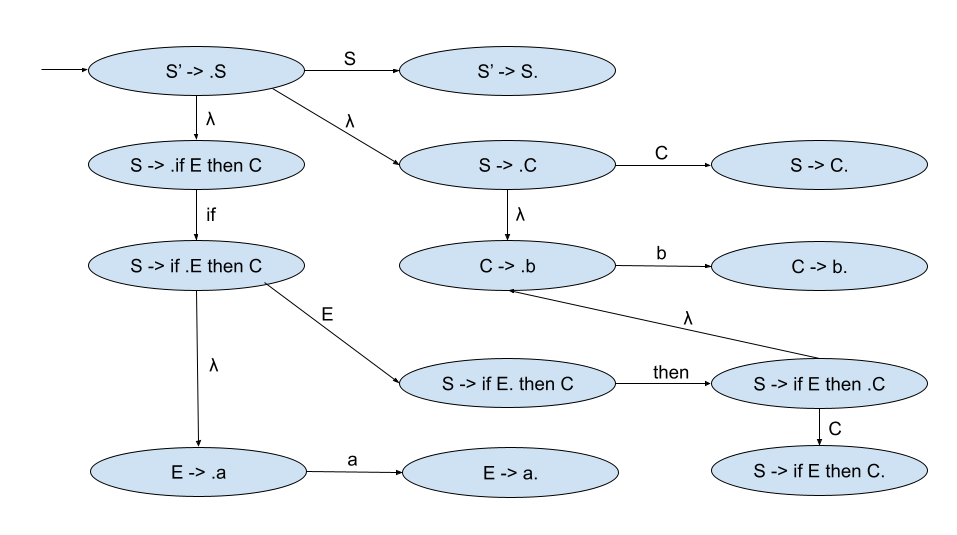
\includegraphics[width=0.5\linewidth]{p2/AFND}
	\caption{AFND da gramática do Ex. 2}
	\label{fig:AFND2}
\end{figure}

Este autômato pode ser transformado no seguinte AF determinístico, visto na figura \ref{fig:AFD2}.

\begin{figure}[htb!]
	\centering
	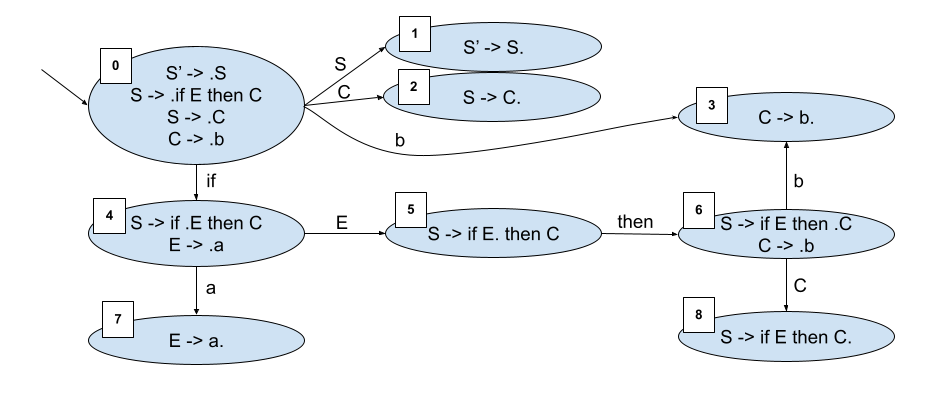
\includegraphics[width=0.5\linewidth]{p2/AFD}
	\caption{AFD da gramática do Ex. 2}
	\label{fig:AFD2}
\end{figure}

Com as informações das regras da gramática, e analisando o autômato, podemos desenvolver a seguinte tabela sintática de análise SLR, descrita na figura \ref{fig:SLR2}.

\begin{figure}[ht!]
	\centering
	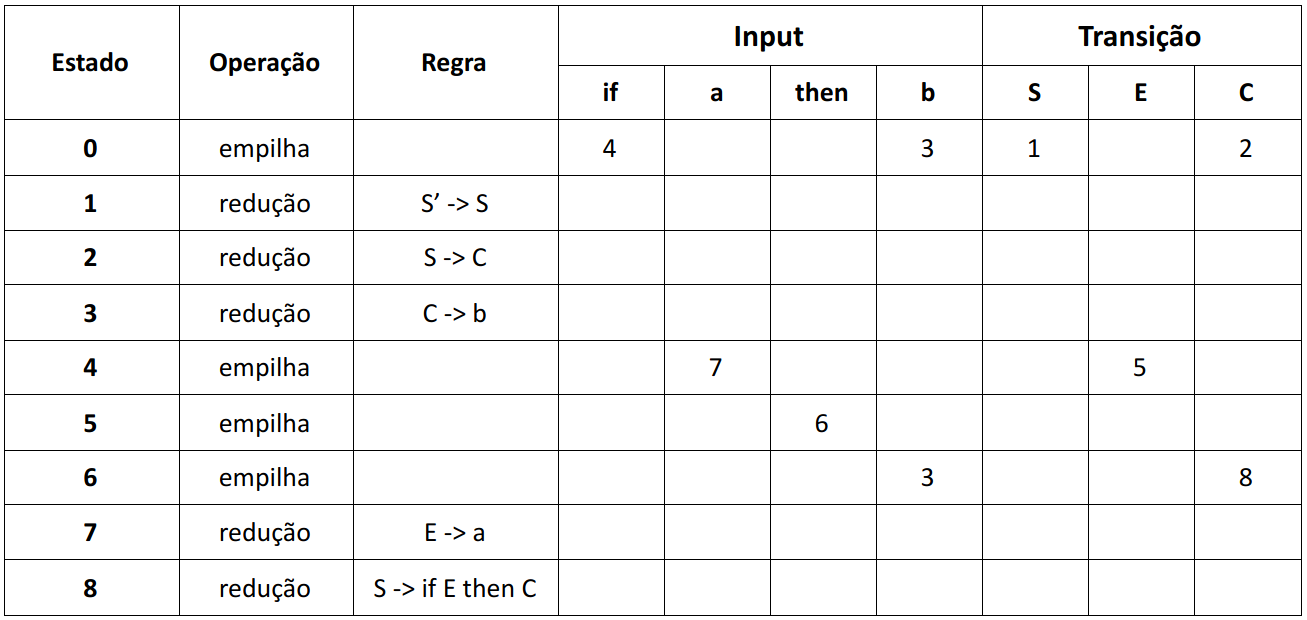
\includegraphics[width=0.7\linewidth]{p2/tabela}
	\caption{Tabela sintática SLR da gramática do Ex. 2}
	\label{fig:SLR2}
\end{figure}

\section{Uma gramática de atributos pode ser utilizada também na fase de geração de código (ver exemplo na questão 5). Neste contexto:}

\subsection{(a) Cite uma desvantagem do uso de gramáticas de atributos para gerar código. }

Uma desvantagem do uso de gramáticas de atributos na geração de código é a possibilidade do alto consumo de memória, visto que a passagem de informações dos nós-folha aos seus ancestrais até a chegada na raiz acaba gerando muitas cópias da cadeia.

\subsection{(b) Cite outro tipo de implementação de geração de código que não utilize a tabela sintática.}

Um tipo de implementação de geração de código que não utiliza a tabela sintática é a solução \textit{ad-hoc}, isto é, ao invés de se utilizar a tabela sintática, podemos fazer a geração de código em conjunto com a análise sintática da cadeia. Ao se amarrar esse processo aos próprios procedimentos sintáticos, evitamos problemas de consumo de memória (citado acima) e complexidade adicional intrínseca as gramáticas de atributos.

\section{Considere a seguinte gramática de atributos para geração de código de 3 endereços:}

\begin{lstlisting}
exp $\rightarrow$  id = exp | aexp
aexp $\rightarrow$ aexp + fator | fator
fator $\rightarrow$ (exp) | num | id
\end{lstlisting}

\begin{figure}[ht!]
	\centering
	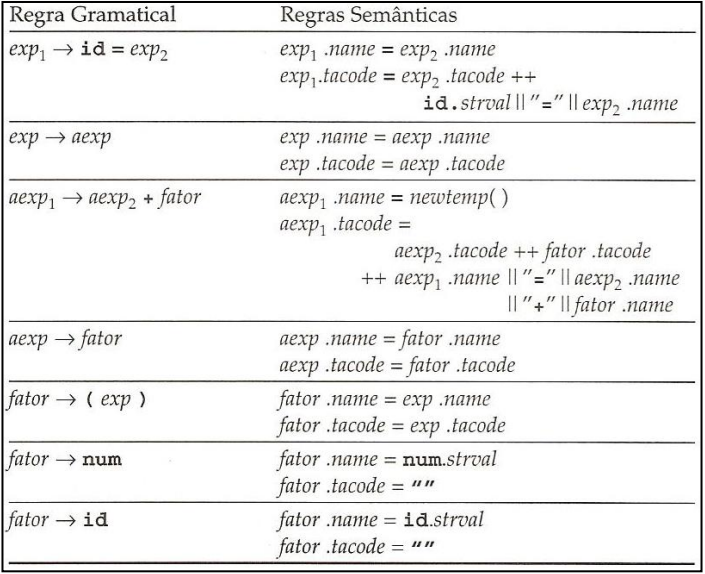
\includegraphics[width=0.5\linewidth]{p2/tabela2.PNG}
\end{figure}

\subsection{Considere que o símbolo || representa concatenação sem pular linha, ++ representa concatenação que pula linha após a operação e strval representa o valor numérico da string. Considere também que newtemp() gera novo nome
temporário, que é guardado no atributo “name”. Mostre a árvore sintática da cadeia \textbf{(x=x+1)+2+y} e mostre o código
de 3 endereços final gerado. Mostre também os códigos gerados nos vértices intermediários da árvore.}

\begin{figure}[ht!]
	\centering
	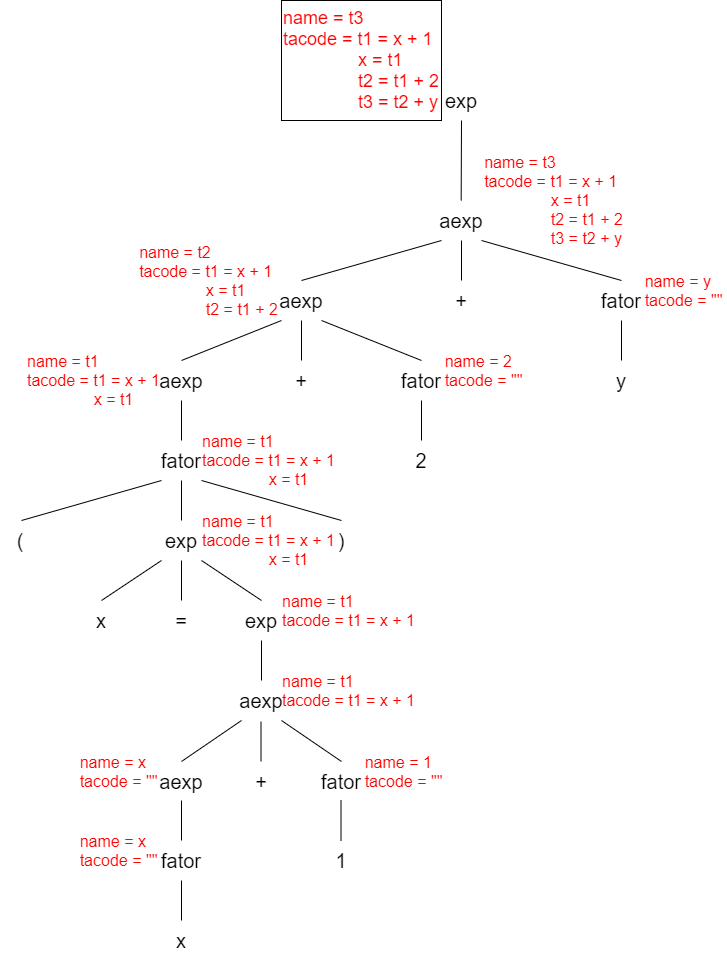
\includegraphics[width=0.8\linewidth]{p2/Q4}
	\caption{Árvore sintática e código de 3 endereços gerado do Ex. 4}
	\label{fig:Q4}
\end{figure}

\end{document}
